\section{Experiments}
\label{sec:experiments}

\subsection{Experimental Setup}
\label{subsec:exp-setup}

\noindent\textbf{Benchmarks and metrics.} We evaluate on three multi-turn agent benchmarks: ALFWorld \citep{shridhar2021alfworld},
WebShop \citep{yao2022webshop}, and Search \citep{jin2025searchr1}. These benchmarks cover embodied household tasks, web shopping, and search-based question answering, allowing us to assess the effectiveness and efficiency of our uncertainty-guided intervention across different environments. We report success rate (SR) on both the seen and unseen splits of ALFWorld, task score and success rate on WebShop, and exact match on four multi-hop Search datasets. Average interaction turns measure efficiency.
Dataset and evaluation details are provided in Appendix~\ref{app:provenance}.

\noindent\textbf{Baselines.} We compare UOPD with four baselines.
\textbf{OPD} \citep{agarwal2024policy,lu2025onpolicydistillation} applies reverse-KL supervision to student-generated actions throughout a rollout.
\textbf{TCOD-F2B} \citep{wang2026exploring} progressively extends the student's rollout horizon from the initial state.
\textbf{TCOD-B2F} \citep{wang2026exploring} starts student rollouts after expert action prefixes and gradually shortens these prefixes to expose the student to earlier decisions.
\textbf{FTB-OPD} \citep{futurebridgeopd2026} introduces teacher corrections at high-disagreement steps and retains them for distillation when they improve teacher preference over subsequent student continuations.

\noindent\textbf{Training details.} On ALFWorld and WebShop, we use Qwen2.5-3B-Instruct and Qwen2.5-1.5B-Instruct \citep{yang2024qwen25} as
students, with task-specific GiGPO-Qwen2.5-7B-Instruct teachers trained
using reinforcement learning  \citep{feng2025gigpo}.
For Search, we distil a base Qwen2.5-1.5B student from
SearchR1-Qwen2.5-7B-em-ppo \citep{jin2025searchr1}. For all methods, we train for $250$ steps on ALFWorld and $150$ on WebShop with
rollout batch size $16$, and for $300$ steps on Search with batch size $64$. For ALFWorld and WebShop, UOPD uses teacher confidence as its uncertainty signal. More training configurations and implementation details are provided in Appendix~\ref{app:provenance}.

\subsection{Main Results}
\label{subsec:exp-alfworld}
\label{subsec:exp-main}

 


We evaluate UOPD’s task performance and efficiency on ALFWorld and WebShop (Table~\ref{tab:exp-agentic})
  and multi-hop question answering (Fig.~\ref{fig:search-15b-multihop}).

\noindent\textbf{UOPD improves task performance and interaction efficiency.}
Across both student sizes, UOPD achieves the highest success rates on the ALFWorld seen and
unseen splits and the highest WebShop scores among the compared distillation methods.
The gains on unseen ALFWorld tasks show that the benefit extends to environments beyond those encountered during training,
while the improvements at $1.5$B demonstrate effective transfer across a larger
teacher--student capacity gap. On WebShop, UOPD raises the $1.5$B student's
score from OPD's $66.3$ to $76.8$ and success rate from $52.3\%$ to $58.6\%$, while reducing
average turns from $7.9$ to $6.8$. UOPD requires the fewest interaction turns in five
of the six evaluation settings, demonstrating its efficiency across tasks and student sizes.

\noindent\begin{minipage}[t]{0.49\textwidth}
\vspace{0pt}
\textbf{The gains extend to multi-hop search.}
Multi-hop search requires the model to retrieve
  relevant evidence and combine it across multiple reasoning
  steps. With a $1.5$B student, UOPD consistently outperforms OPD
  on all four datasets, improving performance by $2.67$–$8.00$
  percentage points, demonstrating the
  benefit of uncertainty-guided supervision for search tasks. Meanwhile, the average number of turns decreases from $5.19$ to $3.90$, indicating
  that improved accuracy is accompanied by higher efficiency at inference time.
\end{minipage}\hfill
\begin{minipage}[t]{0.48\textwidth}
\vspace{0pt}
\centering
\captionsetup{type=figure,skip=3pt}
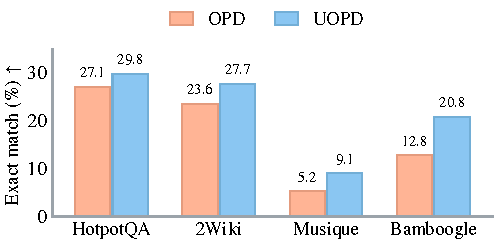
\includegraphics[width=\linewidth]{figures/fig_search_15b_multihop_compact.pdf}
\caption{\textbf{Multi-hop Search results.}}
\label{fig:search-15b-multihop}
\end{minipage}
\par

\vspace{-2.5mm}
\begin{figure}[!htb]
\centering
\captionsetup{skip=3pt}
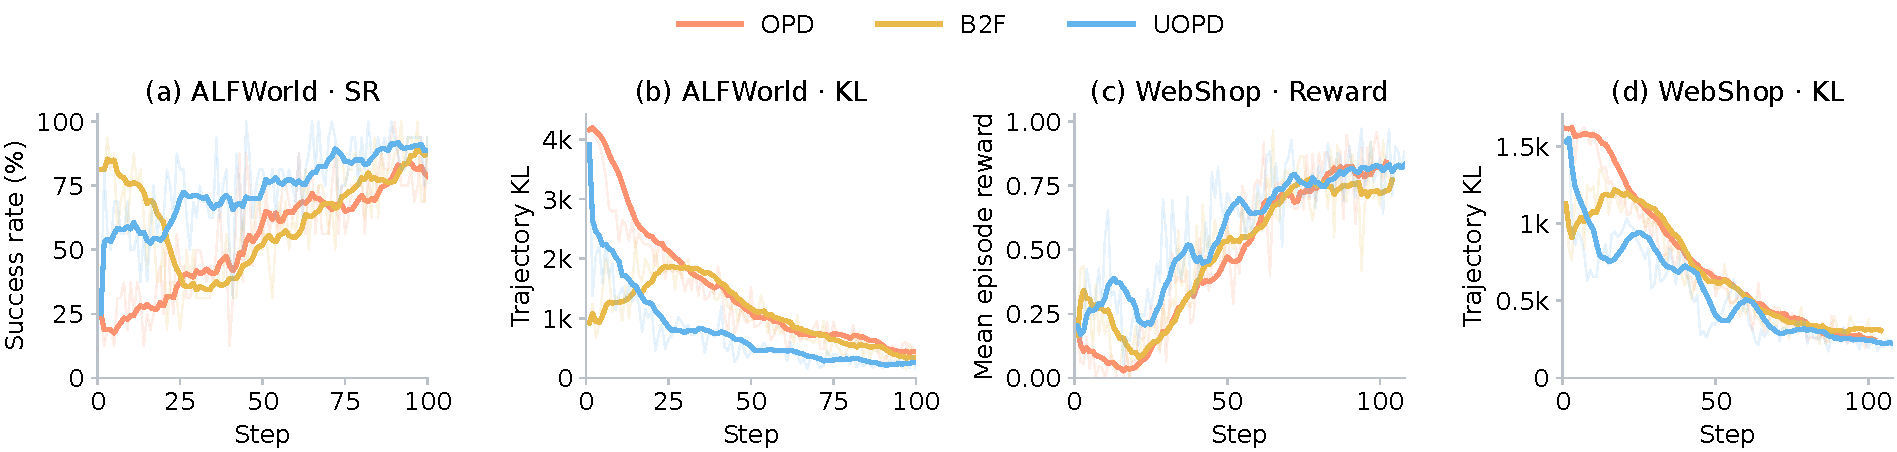
\includegraphics[width=\textwidth]{figures/fig_training_guidance_3b.pdf}
\caption{\textbf{Training dynamics with 3B students.} We compare OPD, TCOD-B2F (B2F),
and UOPD on ALFWorld (a,b: success rate and teacher--student KL) and WebShop
(c,d: reward and teacher--student KL).}
\label{fig:training-guidance}
\end{figure}

\noindent\textbf{Effective guidance during training.}
  Fig.~\ref{fig:training-guidance} shows that UOPD improves
  rollout quality early in training, achieving higher success
  rates on ALFWorld and higher rewards on WebShop than OPD.
  UOPD also exhibits a faster decline in trajectory-level
  teacher--student KL than OPD and B2F. B2F improves initial
  rollout quality through teacher-executed prefixes, but its
  performance drops as these prefixes shorten. This suggests
  that learning from teacher-provided states may not prepare
  the student to execute longer action sequences independently.
  UOPD targets high-uncertainty
  turns throughout the rollout, providing teacher corrections
  while letting the student act and learn throughout the task.

\subsection{Additional Analysis}
\label{subsec:exp-ablation}

Table~\ref{tab:exp-ablation} presents ablation studies with $3$B students on ALFWorld and WebShop,
examining how individual components of UOPD contribute to task performance and interaction efficiency.

\begin{table}[!ht]
\centering
\caption{\textbf{Effects of intervention selection, SFT weight, teacher execution, and schedule
with a 3B student.} The default UOPD configuration uses teacher confidence,
$\beta=1$, teacher execution, and a $30\%\!\to\!5\%$ intervention schedule. Random intervention
samples each turn with the scheduled probability. Values are means over three evaluation seeds, and bold marks the best value
in each column.}
\label{tab:exp-ablation}
\footnotesize
\setlength{\tabcolsep}{4pt}
\begin{tabular*}{\textwidth}{@{\extracolsep{\fill}}l ccccc@{}}
\toprule
& \multicolumn{2}{c}{ALFWorld} & \multicolumn{3}{c}{WebShop} \\
\cmidrule(lr){2-3}\cmidrule(lr){4-6}
Configuration & Seen SR $\uparrow$ & Unseen SR $\uparrow$ & Score $\uparrow$ & SR $\uparrow$ & Turns $\downarrow$ \\
\midrule
\textbf{UOPD} ($\beta=1$, $30\%\!\to\!5\%$) & 90.0 & 88.8 & \textbf{82.4} & \textbf{69.3} & \textbf{6.5} \\
\midrule
\multicolumn{6}{@{}l}{\emph{Intervention signal}} \\
\quad Confidence gap & 89.8 & 87.8 & 77.3 & 69.0 & 7.2 \\
\quad Random intervention & 88.3 & 83.8 & 77.3 & 64.6 & 7.4 \\
\midrule
\multicolumn{6}{@{}l}{\emph{SFT weight}} \\
\quad $\beta=0$ & 86.2 & 80.8 & 79.7 & 66.1 & 6.7 \\
\quad $\beta=0.5$ & 85.7 & 86.3 & 78.0 & 68.0 & 7.3 \\
\quad $\beta=2$ & 89.5 & 86.8 & 77.3 & 68.0 & 7.5 \\
\midrule
\multicolumn{6}{@{}l}{\emph{Teacher execution}} \\
\quad w/o teacher execution & 89.5 & 84.3 & 77.6 & 69.0 & 7.2 \\
\midrule
\multicolumn{6}{@{}l}{\emph{Intervention schedule}} \\
\quad Constant $15\%$ & 90.0 & \textbf{89.6} & 78.0 & 67.7 & 7.0 \\
\quad $50\%\!\to\!30\%$ & \textbf{90.5} & 86.6 & 69.9 & 59.4 & 8.2 \\
\bottomrule
\end{tabular*}
\vspace{-4mm}
\end{table}

\noindent\textbf{Selecting intervention turns.}
We replace uncertainty-based selection with random intervention, sampling each
turn with the same target-rate schedule while retaining teacher execution and
the SFT loss ($\beta=1$). Compared with random intervention, UOPD improves
unseen ALFWorld success from $83.8\%$ to $88.8\%$ and WebShop score from
$77.3$ to $82.4$, while reducing WebShop turns from $7.4$ to $6.5$.
Using the length-normalized student--teacher log-probability gap as the
intervention signal also yields higher success rates than random selection
on both environments. Teacher confidence achieves comparable success rates
while providing higher task scores and shorter interactions on WebShop.

\noindent\textbf{Learning from teacher corrections.}
Removing the SFT loss reduces performance on both benchmarks, with the largest
success-rate drop of $8.0$ percentage points on unseen ALFWorld. Teacher execution
alone therefore does not recover the full benefit of learning from corrections.
The default $\beta=1$ performs best among the tested weights; increasing it to
$\beta=2$ brings no further gains.

\noindent\textbf{Executing teacher corrections.}
On WebShop, teacher execution increases the score from $77.6$ to $82.4$ and
reduces average turns from $7.2$ to $6.5$, while success rates remain similar.
The benefit thus extends beyond whether a task is fully completed: the student
better satisfies the shopping requirements and uses fewer steps per episode.
This suggests that executing corrections during training can complement the
learning signal provided by the SFT loss.

\noindent\textbf{Allocating teacher intervention.}
A higher intervention rate does not consistently improve performance.
The $50\%\!\to\!30\%$ schedule slightly improves seen ALFWorld success but
lowers unseen success and performs worse on WebShop. A constant $15\%$ rate
remains competitive on ALFWorld, achieving the highest unseen success among
the tested schedules, whereas $30\%\!\to\!5\%$ yields the highest score and
fewest turns on WebShop.
See Appendix~\ref{app:telemetry} for intervention dynamics.

\noindent\begin{minipage}[t]{0.49\textwidth}
\vspace{0pt}
\textbf{Training efficiency.}
Fig.~\ref{fig:training-time-3b} compares training time at equal step counts per benchmark. UOPD reduces
training time relative to FTB-OPD by $13.8\%$ on ALFWorld and $36.5\%$ on WebShop,
with $11.5\%$ and $14.7\%$ overhead over OPD. UOPD selects corrections before action
execution, avoiding the paired student continuations used by FTB-OPD to validate
teacher guidance. It thus improves performance with modest training cost compared with standard on-policy distillation.
\end{minipage}\hfill
\begin{minipage}[t]{0.48\textwidth}
\vspace{0pt}
\centering
\captionsetup{type=figure,skip=3pt}
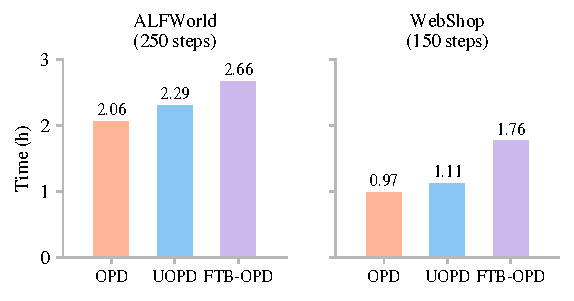
\includegraphics[width=\linewidth]{figures/training_time_3b_preview.pdf}
\caption{\textbf{Training time with 3B students.}}
\label{fig:training-time-3b}
\end{minipage}
\par

\FloatBarrier
